\chapter{The current calculation problem}

In many physical and engineering problems the real interesting variable of the conservation law is the flux inside the domain. The study of micro and nano electronics devices doesn't except this observation and a good description of the current density is a basic requirement.

However we recall that we chose to follow a displacement approach and this implies that the current density is not a variable of the system. Therefore we need to post-processing the carrier solutions in order to reconstruct the current density of electrons and holes.

It will be reather regrettable to lost the accuracy of our results during this computation, for this reason in this chapter we investigate some techniques in order to compute a correct current density inside the device.



\section{Drift-Diffusion formula}

In section \ref{sec: carrier transport} we saw that exist three way to represent the current density, but due to numerical issues not all of them perform a good approximation. As example we exluded from our analysis the \textit{Slotboom equations} \referenzaeq{eq: Jn slotboom} \referenzaeq{eq: Jp slotboom} because  the exponential dependency by the factor $\varphi / V_{th}$ brings unavoidable numerical instability. 
The classical \textit{Drift-Diffusion formula} \referenzaeq{eq: drift diff electron} \referenzaeq{eq: drift diff hole} presents also some difficulties: the drift and the diffusion contributions are respectively well defined but the combination of them brings often problematic oscillations.

Let us introduce some useful notations: with the subscript $K$  we refer to a quantity defined on elements, while the $h$ subscript refers to a quantity defined on vertices. The solutions $\varphi_h$, $n_h$ and $p_h$ obtained with the discretization scheme presented in chapter \ref{sec: Numerical approximation} are linear continuous functions. Accordingly to  \referenzaeq{eq: drift diff electron} and \referenzaeq{eq: drift diff hole},  in order to compute $\vect{J}_n$ and $\vect{J}_p$ numerical derivatives of the solutions must be done. As a consequence in this framework the discrete current densities live in different discretized spaces, indeed they are naturally constant element piecewise functions ($\vect{J}_{n},\vect{J}_{p} \in [X_h^0]^3$). If we want combine solutions and their derivatives, we have to compute appropriate projection of $n_h$ and $p_h$
 
 \begin{align*}
 n|_K := <n_h> \\ 
p|_K := <p_h>
 \end{align*}

where with the symbol $<\cdot >$ we refer to a suitable average on the element, for example this operation could be the standard integral or the armonic average. If the diffusion and the mobility coefficients are variable functions of the space and defined on vertices they also have to be projected on the space $X_h^0$.

We implemented a numerical derivation based on the Lagrange polynomial interpolator of the first order

\begin{equation}
\nabla n \simeq \nabla (\Pi^1_h n) = \sum_{i=1}^{N_h} n_i \nabla \psi_i = \nabla n_h
\end{equation}
 
Notice that $\nabla n_h \in X_h^0$.
The discretized form of the equations \referenzaeq{eq: Jn DD}, \referenzaeq{eq: Jp DD} reads as

\begin{align}
\vect{J}_n|_K &= -qn|_K\mu_n\nabla \varphi + qD_n n|_K\nabla n_h \label{eq: Jn DD discrete}\\ 
\vect{J}_p|_K &= -qp|_K\mu_p\nabla \varphi - qD_p p|_K \nabla p_h \label{eq: Jp DD discrete} 
\end{align}
 
 for the sake of the simplicity we consider only constat diffusion and mobility coefficients.
%  \referenzaeq{eq: Jn qf} and \referenzaeq{eq: Jp qf}
%\vect{J}_n^k &= -q<n>\mu_n\nabla \varphi_n \label{eq: Jn qf discrete}\\
%\vect{J}_p^k &= -q<p>\mu_p\nabla \varphi_p \label{eq: Jp qf discrete}

Equations \referenzaeq{eq: Jn DD discrete} and \referenzaeq{eq: Jp DD discrete} can be easily computed over each elements of $\mathcal{T}_h$, but the results are often bad. 
 
 \textcolor{red}{Aggiungere figure dei contributi drift a diffusion separati e del bilancio oscillante per un caso semplice come il diodo. Aggiungere inoltre un caso con il MOS n-channel che verr\`a confrontato con le modifiche apportate dalla formula nella sezione upwinding.}
%\begin{figure}[!h]
%\centering
%
%\subfloat[][\emph{Jn}]
%{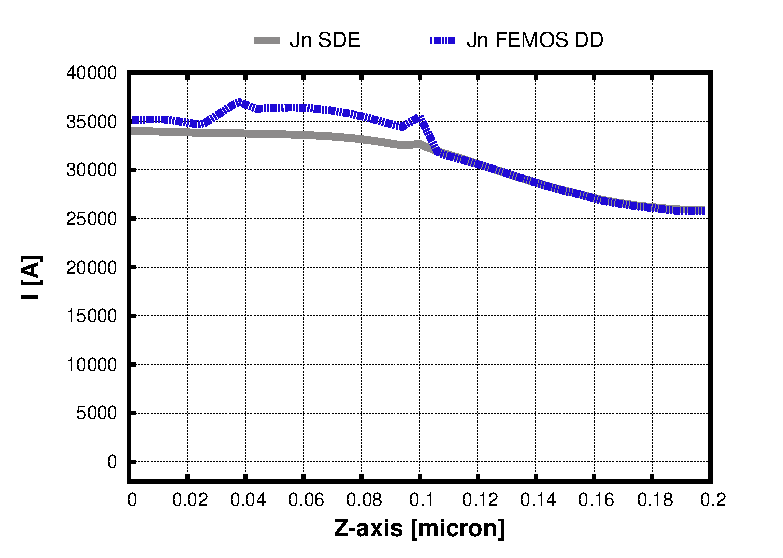
\includegraphics[height=4.5cm]{Corrente/ConfrontiCorrentiBulkJN_SDEVsDD.eps}}
%\subfloat[][\emph{Jp}]
%{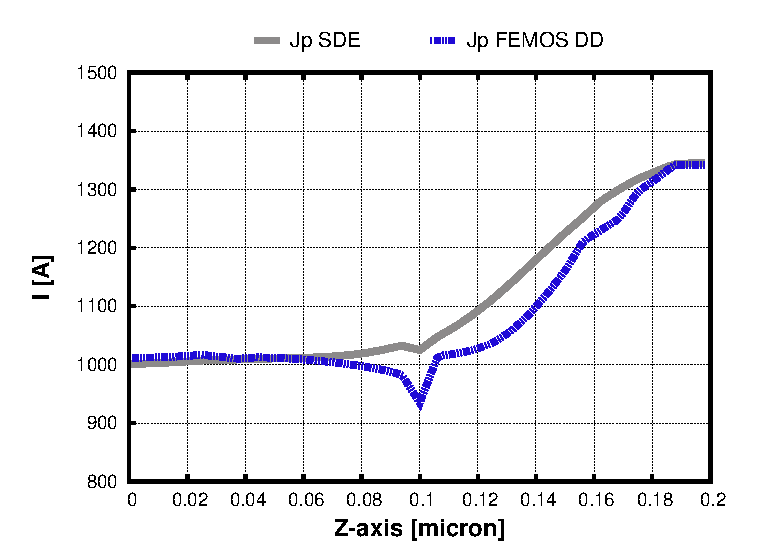
\includegraphics[height=4.5cm]{Corrente/ConfrontiCorrentiBulkJP_SDEVsDD.eps}}
%
%\subfloat[][\emph{Jn}]
%{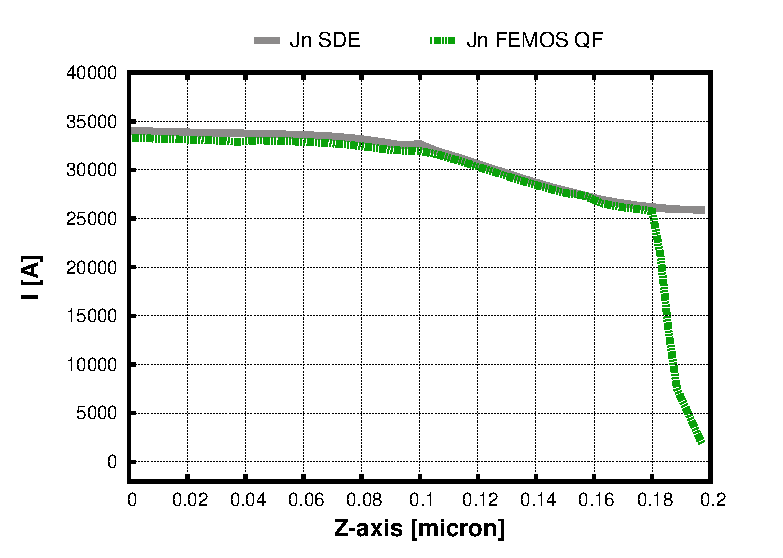
\includegraphics[height=4.5cm]{Corrente/ConfrontiCorrentiBulkJN_SDEVsQF.eps}}
%\subfloat[][\emph{Jp}]
%{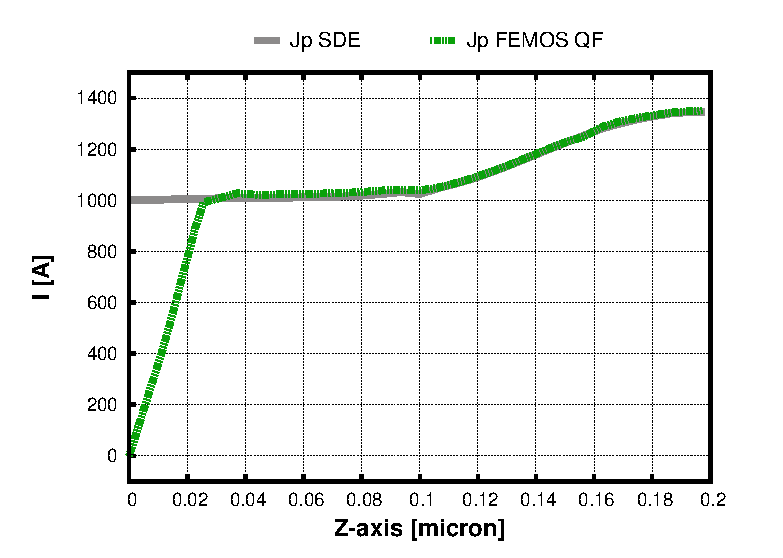
\includegraphics[height=4.5cm]{Corrente/ConfrontiCorrentiBulkJP_SDEVsQF.eps}}
%
%
%\end{figure} 
 

%\begin{figure}[!h]
%\centering
%
%\subfloat[][\emph{Jn}]
%{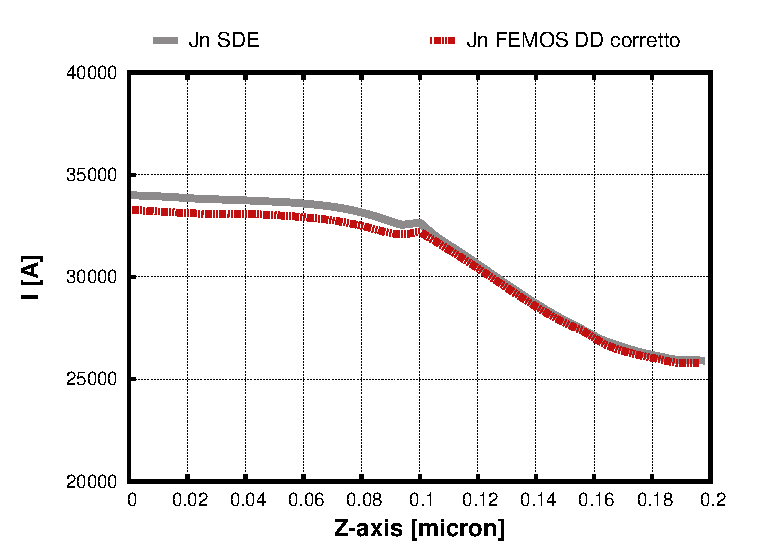
\includegraphics[height=4.5cm]{Corrente/ConfrontiCorrentiBulkJN_SDEVsDDcorretto.eps}}
%\subfloat[][\emph{Jp}]
%{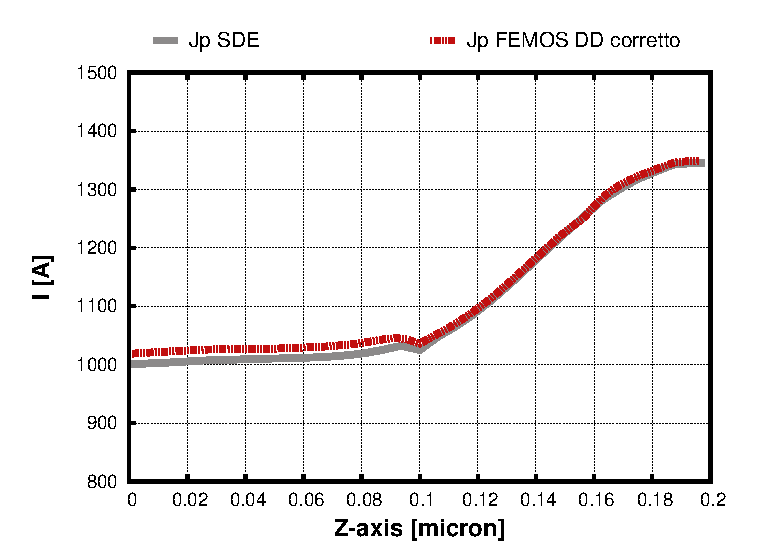
\includegraphics[height=4.5cm]{Corrente/ConfrontiCorrentiBulkJP_SDEVsDDcorretto.eps}}
%
%\subfloat[][\emph{Jn}]
%{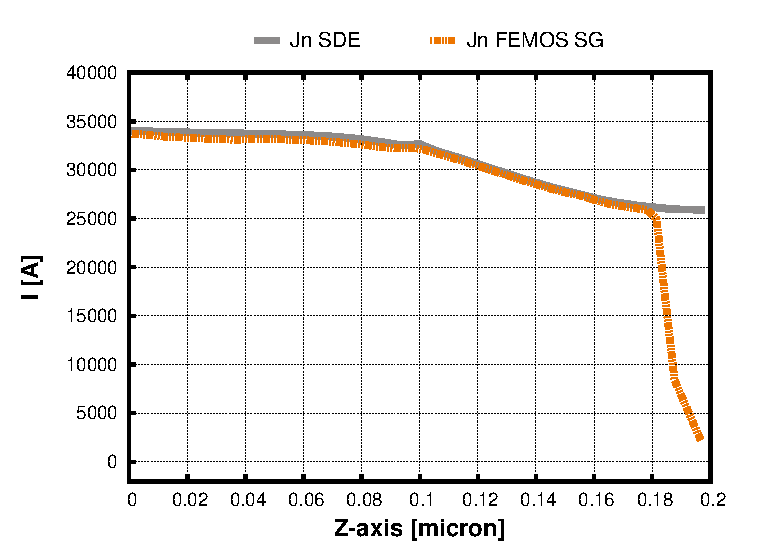
\includegraphics[height=4.5cm]{Corrente/ConfrontiCorrentiBulkJN_SDEVsSG.eps}}
%\subfloat[][\emph{Jp}]
%{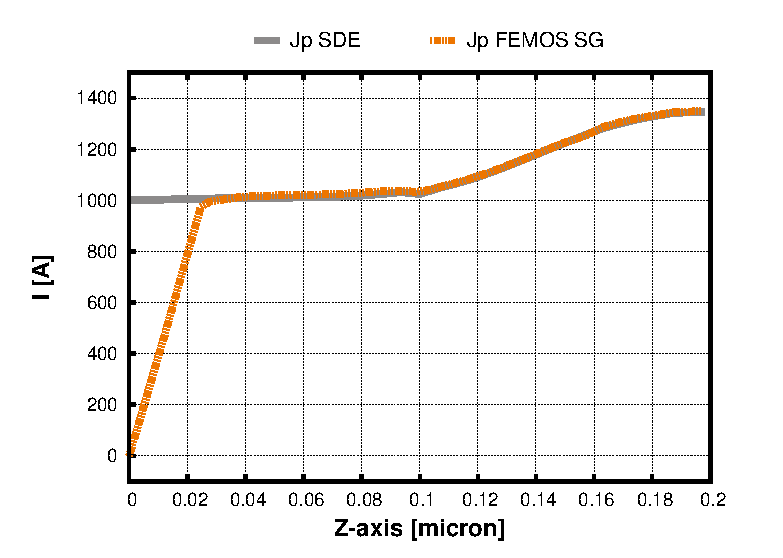
\includegraphics[height=4.5cm]{Corrente/ConfrontiCorrentiBulkJP_SDEVsSG.eps}}
%
%
%\end{figure} 

 
 
 \clearpage
 
 
 
 
 
\section{Edge average techiniques} 
 
 It's well known that the classical Scharfetter-Gummel scheme for discretizing drift-diffusion models has proven  itself to be the workhorse for semiconductor device modeling codes, indeed the EAFE scheme proposed in section \ref{sec: continuity equations} is strictly related to the FVSG (Finite Volume Scharfetter-Gummel) method presented by Bank, Fichtner and Rose \cite{Bank:FVSG}. 

In this section we exposed briefly the Scharfetter-Gummel formula for  a one spatial domain and we reported the extension for the 2D proposed in \cite{Bank:FEvsBOX}. Finally we present an innovative method in order to extend the Scharfetter-Gummel approach to the 3D framework.

\subsection{Scharfetter-Gummel 1D}

Consider the resolution of the continuity equation along a monodimensional domain. For the sake of simiplicity we contemplate a uniform partition (this hypotesis is not necessary for a more generic analysis). Moreover on every nodes is defined the electrostatic potential $\varphi$, and on every elements the relative electrostatic field $\vect{E}$. In order to avoid redundant considerations and calculuses, we proceed with our analysis considering only the current density of electrons ($\vect{J}_n$).

 In 1969 D. Scharfetter and H.K. Gummel (two scientists of Bell Labs), introduced a formula to compute the current density in this case, given $\varphi$ and the density solution ($n$) on every nodes. This innovative approach led for the twenty years to follow every simulation which contemplates electric-devices. 
 
We know that the constituve law is composed by a drift component, which depends on the electric field, and a diffusion component, which depends on the variation of the carrier density. Consider a generic element $K$, we define the drop in voltage $\Delta \varphi^k=\varphi_{i+1}-\varphi_{i}$. There are three possible situations which are well explain in \figref{fig: SF figure}:
\begin{itemize}
\item $\Delta \varphi \gg0$, mainly drift component from right to left 
\item $\Delta \varphi \ll0$, mainly drift component from left to right
\item $\Delta \varphi \simeq 0$, mainly diffusion component
\end{itemize} 
 
 
\begin{figure}[!h]
\centering
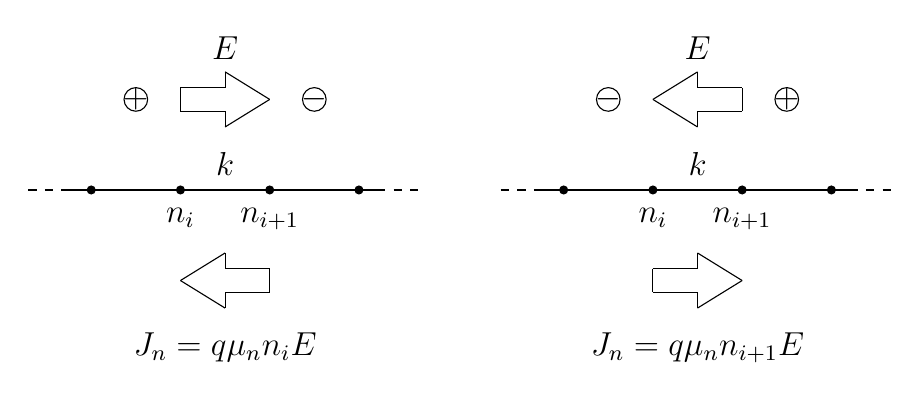
\begin{tikzpicture}
[scale=1.0]
%Solid line
\def\ax{0.5}
\def\ay{0}
\def\bx{4.5}
\def\by{0}

\def\delta{0.3}

%Dash line
\def\cx{0}
\def\cy{0}
\def\dx{5}
\def\dy{0}

\def\Np{3}
\def\step{\bx/\Np-\ax/\Np-2*\delta/\Np}
\def\halfstep{0.5*\bx/\Np-0.5*\ax/\Np-\delta/\Np}

\draw [dashed] (\cx,\cy)--(\dx,\dy);
\draw [thick](\ax,\ay)--(\bx,\by);

\draw [black,draw, fill=black] (\ax+\delta,\ay) circle [radius=0.05];
\draw [black,draw, fill=black] (\ax+\delta+\step,\ay) circle [radius=0.05];
\draw [black,draw, fill=black] (\ax+\delta+\step+\step,\ay) circle [radius=0.05];
\draw [black,draw, fill=black] (\ax+\delta+\step+\step+\step,\ay) circle [radius=0.05];

\draw [thick] (\ax+\delta +\step+\halfstep,\ay+0.05) node[above]{\large $k$};
\draw [thick] (\ax+\delta+\step,\ay-0.1) node[below]{\large $n_{i}$};
\draw [thick] (\ax+\delta+\step + \step,\ay-0.1) node[below]{\large $n_{i+1}$};


\draw [black,draw] (\ax+\delta+\halfstep,\ay+1.15) circle [radius=0.15];
\draw [black,draw] (\ax+\delta+\step + \step + \halfstep,\ay+1.15) circle [radius=0.15];
\node at (\ax+\delta + \halfstep,\ay+1.15){\large $+$};
\node at (\ax+\delta +\step + \step + \halfstep,\ay+1.15){\large $-$};

\node at (\ax+\delta +\step + \halfstep,\ay+1.8){\large $\vect{E}$};
\node at (\ax+\delta +\step + \halfstep,\ay-2.0){\large $\vect{J}_n=q\mu_n n_{i}\vect{E}$};

%Freccia
\draw (\ax+ \delta + \step,\ay+1)--(\ax+\delta+\step+\halfstep,\ay+1);
\draw (\ax+\delta + \step,\ay+1.3)--(\ax+\delta+\step+\halfstep,\ay+1.3);
\draw (\ax+\delta+ \step,\ay+1)--(\ax+\delta+\step,\ay+1.3);
\draw (\ax+\delta + \step +\halfstep,\ay+1.3)--(\ax+\delta+\step+\halfstep,\ay+1.5);
\draw (\ax+\delta + \step +\halfstep,\ay+1)--(\ax+\delta+\step+\halfstep,\ay+0.8);
\draw (\ax+\delta + \step +\halfstep,\ay+1.5)--(\ax+\delta+\step+\step,\ay+1.15);
\draw (\ax+\delta + \step +\halfstep,\ay+0.8)--(\ax+\delta+\step+\step,\ay+1.15);

%Freccia
\draw (\ax+ \delta + \step +\halfstep,\ay-1)--(\ax+\delta+\step +\step,\ay-1);
\draw (\ax+\delta + \step + \halfstep,\ay-1.3)--(\ax+\delta+\step + \step,\ay-1.3);
\draw (\ax+\delta+ \step + \step,\ay-1)--(\ax+\delta+\step+\step,\ay-1.3);

\draw (\ax+\delta + \step +\halfstep,\ay-1.3)--(\ax+\delta+\step+\halfstep,\ay-1.5);
\draw (\ax+\delta + \step +\halfstep,\ay-1)--(\ax+\delta+\step+\halfstep,\ay-0.8);
\draw (\ax+\delta + \step +\halfstep,\ay-1.5)--(\ax+\delta+\step,\ay-1.15);
\draw (\ax+\delta + \step +\halfstep,\ay-0.8)--(\ax+\delta+\step,\ay-1.15);


%Solid line
\def\ax{6.5}
\def\ay{0}
\def\bx{10.5}
\def\by{0}

\def\delta{0.3}

%Dash line
\def\cx{6}
\def\cy{0}
\def\dx{11}
\def\dy{0}

\def\Np{3}
\def\step{\bx/\Np-\ax/\Np-2*\delta/\Np}
\def\halfstep{0.5*\bx/\Np-0.5*\ax/\Np-\delta/\Np}

\draw [dashed] (\cx,\cy)--(\dx,\dy);
\draw [thick](\ax,\ay)--(\bx,\by);

\draw [black,draw, fill=black] (\ax+\delta,\ay) circle [radius=0.05];
\draw [black,draw, fill=black] (\ax+\delta+\step,\ay) circle [radius=0.05];
\draw [black,draw, fill=black] (\ax+\delta+\step+\step,\ay) circle [radius=0.05];
\draw [black,draw, fill=black] (\ax+\delta+\step+\step+\step,\ay) circle [radius=0.05];

\draw [thick] (\ax+\delta +\step+\halfstep,\ay+0.05) node[above]{\large $k$};
\draw [thick] (\ax+\delta+\step,\ay-0.1) node[below]{\large $n_{i}$};
\draw [thick] (\ax+\delta+\step + \step,\ay-0.1) node[below]{\large $n_{i+1}$};

\draw [black,draw] (\ax+\delta+\halfstep,\ay+1.15) circle [radius=0.15];
\draw [black,draw] (\ax+\delta+\step + \step + \halfstep,\ay+1.15) circle [radius=0.15];
\node at (\ax+\delta + \halfstep,\ay+1.15){\large $-$};
\node at (\ax+\delta +\step + \step + \halfstep,\ay+1.15){\large $+$};

\node at (\ax+\delta +\step + \halfstep,\ay+1.8){\large $\vect{E}$};
\node at (\ax+\delta +\step + \halfstep,\ay-2.0){\large $\vect{J}_n=q\mu_n n_{i+1}\vect{E}$};

%Freccia
\draw (\ax+ \delta + \step +\halfstep,\ay+1)--(\ax+\delta+\step +\step,\ay+1);
\draw (\ax+\delta + \step + \halfstep,\ay+1.3)--(\ax+\delta+\step + \step,\ay+1.3);
\draw (\ax+\delta+ \step + \step,\ay+1)--(\ax+\delta+\step+\step,\ay+1.3);
\draw (\ax+\delta + \step +\halfstep,\ay+1.3)--(\ax+\delta+\step+\halfstep,\ay+1.5);
\draw (\ax+\delta + \step +\halfstep,\ay+1)--(\ax+\delta+\step+\halfstep,\ay+0.8);
\draw (\ax+\delta + \step +\halfstep,\ay+1.5)--(\ax+\delta+\step,\ay+1.15);
\draw (\ax+\delta + \step +\halfstep,\ay+0.8)--(\ax+\delta+\step,\ay+1.15);

%Freccia
\draw (\ax+ \delta + \step,\ay-1)--(\ax+\delta+\step+\halfstep,\ay-1);
\draw (\ax+\delta + \step,\ay-1.3)--(\ax+\delta+\step+\halfstep,\ay-1.3);
\draw (\ax+\delta+ \step,\ay-1)--(\ax+\delta+\step,\ay-1.3);
\draw (\ax+\delta + \step +\halfstep,\ay-1.3)--(\ax+\delta+\step+\halfstep,\ay-1.5);
\draw (\ax+\delta + \step +\halfstep,\ay-1)--(\ax+\delta+\step+\halfstep,\ay-0.8);
\draw (\ax+\delta + \step +\halfstep,\ay-1.5)--(\ax+\delta+\step+\step,\ay-1.15);
\draw (\ax+\delta + \step +\halfstep,\ay-0.8)--(\ax+\delta+\step+\step,\ay-1.15);

\end{tikzpicture}

\caption{Effect of high electric field over the current density of electron.}
\label{fig: SF figure}
\end{figure}


With the $Sharfetter-Gummel$ formula it's possibile taking into account every of these situations and solve boundary layer problems which occurs often in presence of strong drift component contribute.

 \begin{equation}
\label{eq: scharfetter gummel 1D electron}
J_n^k=q\frac{D_n}{h}
\left[ n_{i+1}\mathcal{B}\left(\frac{\Delta \varphi^k}{V_{th}}\right)- n_i\mathcal{B}\left(-\frac{\Delta \varphi^k}{V_{th}}\right)\right]  
\end{equation}

In the latter case $\Delta \varphi=0$ the formula became:

\begin{equation}
J_n^k=qD_n\frac{n_{i+1}-n_{i}}{h}
\end{equation}

which is the correct approximation of the current density using $\mathbb{P}_1$ basis. 

\subsection{Scharfetter-Gummel 2D}

One of the main results presented in \cite{Bank:FEvsBOX} is the equivalence between the finite volume and Galerkin discretizations of the continuity equation. In order to facilitate the connection between these different discretization approaches the authors introduced for each $K \in \mathcal{T}_h$ a linear map $\mathcal{J}_{K}:\mathbb{R}^3\rightarrow\mathbb{R}^2$ defined by

\begin{equation}
\label{eq: map current}
\mathcal{J}_{K}(\{\gamma_i\}_{i=1}^3) = \dfrac{1}{|K|}\sum_{i=1}^3 \gamma_i |e_i| s_i \vect{t}_i
\end{equation}

where $s_i$ is the meausure of the segment from the midpoint  of $e_i$ to the intersection of the perpendicular edge bisectors and $\vect{t}_i$ denote the unit tangent vector of the edge $e_i$.
$\mathcal{J}_K$ has the following properties:
\begin{align}
\mathcal{J}_K(\{\vect{J}\cdot \vect{t}_i\}_{i=1}^3) & = \vect{J} \label{eq: map is current} \\
 \mathcal{J}_K(\{s_i^{-1}\}_{i=1}^3) & = 0 \\
 \int_K \mathcal{J}_K(\{\gamma_i\}_{i=1}^3) \cdot \nabla \psi \, dK & = \gamma_{i+1}s_{i+1} - \gamma_{i-1}s_{i-1}
\end{align}
 
 Equation \referenzaeq{eq: map is current} says that if we are able to compute the tangential componente of the current density over all edges, we can combine those values accordingly with \referenzaeq{eq: map current} and obtain the total current density $\forall K \in \mathcal{T}_h$.
 
 We already introduced a formula for the computation of $\vect{J}\cdot \vect{t}_i$ in section \ref{sec: continuity equations}, indeed for the EAFE scheme in the case of electron we have
 
\begin{equation}
\label{eq: EAFE edge formula}
\small
\vect{J}\cdot \vect{t}_i = j_{e_i} = \mathcal{H}_{e_i}(qD_n e^{(\varphi/V_{th})}) \dfrac{\mathcal{B}(\delta_i(\varphi / V_{th}))n_{h,k} -  \mathcal{B}(-\delta_i(\varphi / V_{th}))n_{h,j}}{|e_i|}
\end{equation}

similarly for the classical FVSG scheme this contribution is defined as

\begin{equation}
\vect{J}\cdot \vect{t}_i = j_{e_i}  = \mathcal{H}_{e_i}(qD_n e^{(\varphi/V_{th})}) \nabla (e^{-\varphi / V_{th}}n_h) \cdot \vect{t}_i
\end{equation}

where for both $\varphi$ is the solution of the electrostatic potential given by the resolution of the non linear poisson equation.

%Again the Sharfetter-Gummel formula play a lead role in \referenzaeq{eq: EAFE edge formula}
The extension of this procedure to the 3D case is not trivial: the meaning of the cross-section $s_i$ becomes more involved and equation \referenzaeq{eq: map current} is a sum over six edges rather than three which lead to increasing computational costs and possible numerical instabilities.


\subsection{Scharfetter-Gummel 3D}
\label{sec: SG 3D} 
 
In the previous sections we have discussed the goodness of the Sharfetter-Gummel formula, but in the 2D case we see also that the computation of the total current density becomes more complex as the dimension of the simulation increases. In this section we present and validate an innovative method which can go beyond the above limitations.

Without loss of generality we show the procedure only for the electron continuity equation.
We recall here the quasi fermi formula for the electron current density:

\begin{equation}
\label{eq: current density fermi}
\vect{J}_n=-q \mu_n n \nabla \varphi_n
\end{equation}

\referenzaeq{eq: current density fermi} can be rewritten considering equation \referenzaeq{eq: non eq n density mb}:

\begin{equation}
\label{eq: current density canonic form}
\vect{J}_n\dfrac{ exp\left(\dfrac{\varphi_n-\varphi}{V_{th}}\right)}{q \mu_n n_i} + \nabla \varphi_n = 0
\end{equation}

Let be $\vect{J}_n\in[L^2(\Omega)]^3$ and $\varphi_n,\varphi \in H^1(\Omega)$. We are able to multiply \referenzaeq{eq: current density canonic form} with a generic function $\vect{q}\in[L^2(\Omega)]^3$ and then intagrate over the domain $\Omega$:

\begin{equation}
\label{eq: variation form of current density continuos}
\int_\Omega \dfrac{ exp \left( \dfrac{\varphi_n-\varphi}{V_{th}} \right) }{q \mu_n n_i} \vect{J}_n \cdot \vect{q} \, d\Omega
 + \int_\Omega \nabla \varphi_n \cdot \vect{q} \, d\Omega = 0 
\end{equation}


We proceed taking the usual discrete space of the constant elemenwise functions:

\begin{equation}
\label{eq: spaces elementwise constant}
V_h=\left\{ w \in L^2(\Omega) : w|_{K}\in \mathbb{P}_0 \forall K \in \tau_h\right\}
\end{equation}

Now the discrete quantitaties are $\vect{J}_n^h\in[V_h]^3$ and $\nabla \varphi_n^h \in V_h$. We consider the following choice of the test function $\vect{q}_h \in [V_h]^3$:

\begin{equation}
\label{eq: form of qh}
\vect{q}^h_{1,2,3} = \left\{ \begin{bmatrix} 1 \\ 0 \\ 0 \end{bmatrix}  \begin{bmatrix} 0 \\ 1 \\ 0 \end{bmatrix}  \begin{bmatrix} 0 \\ 0 \\ 1 \end{bmatrix}  \right\}
\end{equation}

From \referenzaeq{eq: variation form of current density continuos} we obtain a system of equations defined for each $K \in \mathcal{T}_h$:

\begin{equation}
\label{eq: variation form of current density}
\int_K \dfrac{ exp \left( \dfrac{\varphi_n-\varphi}{V_{th}} \right) }{q \mu_n n_i} \vect{J}_n^h \cdot \vect{q}^h_i \, dK
 + \int_K \nabla \varphi_n^h \cdot \vect{q}^h_i \, dK = 0 \psp{10} \forall i=1,2,3
\end{equation}

After the intagration we obtain the formula for the generic component of the current density:

\begin{equation}
\label{eq: first formula for J}
[\vect{J_n}]_i = - \mathcal{H}_K \left( q \mu_n n_i exp \left( \dfrac{\varphi-\varphi_n}{V_{th}} \right)  \right) \dfrac{\partial \varphi_n^h}{\partial x_i} \psp{5} i = 1...d \psp{5} \forall K \in \tau_h
\end{equation}

We have no intention to resolve the armonic average with a comlete 3D integration which may be expensive in calculation time. Therefore we suppose that there is an edge of $K$ such that 

\begin{equation}
\label{eq: approzimation from 3D to edge}
\left(\dfrac{\int_K f^{-1} \, dK}{|K|} \right)^{-1} \simeq \left(\dfrac{\int_{e*} f^{-1} \, de}{|e^*|} \right)^{-1}
\end{equation}
 
 where $f=q \mu_n n_i exp((\varphi-\varphi_n)/V_{th})$.
  We are assuming that the diffusive coefficient could be predicted if we consider only the edge where the phenomena is more significative rather than the entire element. In order to define which is the correct edge consider a quantity defined on the verteces

\begin{equation}
\label{eq: differenza tra pot e qf}
\Phi := \varphi - 	\varphi_n
\end{equation}

which is the difference between the electrostatic potential and the quasi fermi potential level. Now for every element consider two vertices: $\vect{x}_m$ s.t. $\Phi(\vect{x}_m)=\Phi_m := min_K(\Phi)$ and $\vect{x}_M$ s.t. $\Phi(\vect{x}_M)=\Phi_M:=max_K(\Phi)$. Obviously it exists only one edge which connects these two points and on this one we perform the 1D integration \referenzaeq{eq: approzimation from 3D to edge}.

%\begin{equation}
%\left(\dfrac{1}{|e^*|} \int_{e*} \dfrac{   exp \left( %\dfrac{\varphi_n-\varphi}{V_{th}} \right) }{ q \mu_n n_i} \, de %\right)^{-1}
%\end{equation}


Along the edge $e^*$ we can consider

\begin{equation}
f(s) = q \mu_n n_i exp\left( \Phi_m + (\Phi_M-\Phi_m)\dfrac{s-s_m}{|e^*|} \right)
\end{equation}

where $s \in [s_m,s_M]$ is the parameter refered to the edge $e^*$ s.t. $f(s_m)=f(\vect{x}_m)$ and $f(s_M)=f(\vect{x}_M)$. We can solve \referenzaeq{eq: approzimation from 3D to edge} with the following change in variable

\begin{equation*}
\eta := \dfrac{s-s_m}{|e^*|}
\end{equation*}

and proceed with trivial integration steps

\begin{align*}
\int_{e^*} f^{-1} \, de & = |e^*| \int_0^1 \dfrac{exp \left(-\Phi_m - (\Phi_M-\Phi_m)\eta \right)}{q\mu_n n_i} 
 \, d\eta \\
  & = |e^*|\dfrac{exp (-\Phi_m)}{q\mu_n n_i} \dfrac{exp ( \Phi_m-\Phi_M)-1}{\Phi_m-\Phi_M} \\
 & =  |e^*|\dfrac{exp (-\Phi_m)}{q\mu_n n_i} \dfrac{1}{\mathbf{B}(\Phi_m-\Phi_M)}
\end{align*}

finally we obtain

\begin{equation}
\label{eq: finally approzimation 3D to 1D}
\int_{K} f^{-1} \, dK \simeq  q \mu_n n_i exp(\Phi_m) \mathbf{B}(\Phi_m-\Phi_M)
\end{equation}

Similar results may be obtained repeating the integration and considering $s_M$ as start point:

\begin{equation}
\label{eq: approssimazione sm}
\int_{K} f^{-1} \, dK \simeq  q \mu_n n_i exp(\Phi_M) \mathbf{B}(\Phi_M-\Phi_m)
\end{equation}

Equation \referenzaeq{eq: finally approzimation 3D to 1D} and \referenzaeq{eq: approssimazione sm} can be combined and find

\begin{equation}
\label{eq: first formula for J}
\vect{J}_n|_K = -  q \mu_n  \left[ \dfrac{ n_{min} \mathbf{B}(-\Delta \Phi_{max})  + n_{max}\mathbf{B}(\Delta \Phi_{max})}{2} \right]\nabla \varphi_n^h
\end{equation}

where $n_{min}=n_i e^{\Phi_m}$ and $n_{max}=n_i e^{\Phi_M}$.

If we consider equation \referenzaeq{eq: first formula for J} over a one spatial domain we can recover equation \referenzaeq{eq: scharfetter gummel 1D electron}, then we can say that this approach is the natrual extension of the $Sharfetter-Gummel$ formula for the 3D case.




\section{Upwinding techiniques}

It's well known that classical finite element method is unstable when the P\`eclet number ($\mathbb{P}e$) is large. Coefficient $\mathbb{P}e$ includes the influence of the drift component and is proportional to the product $|\nabla \varphi| h$. Therefore the presence of boundary layers for the electrostatic potential makes problematic the resolution of the continuity equation. This has led to the use of upwind finite element techniques: in one spatial domain this contribution is written as artificial diffusion term which modifies the convection diffusion equation. Generally speaking we can define a function $\Phi$ of the P\`eclet number such that

\begin{align}
\label{eq: consistenza}
\lim_{h \to 0} \Phi = 0
\end{align}

The perturbed problem in the case of the electron continuity equation becomes

\begin{equation}
\label{eq: perturbed problem}
- \nabla \cdot (qD_n(1+\Phi)\nabla n - q \mu_n n \nabla \varphi) = -qR
\end{equation}

Similarly the new weak form is

\begin{equation}
\label{eq: weak form perturbed}
a_h(n,v) = a(n,v) + \int_{\Omega} \Phi \nabla n \cdot \nabla v \, d\Omega
\end{equation}

Property \referenzaeq{eq: consistenza} is fundamental in order to guarantee the consistence of \referenzaeq{eq: weak form perturbed} with respect to the standard Galerkin weak form.

Considering the framework just presented the \textit{Sharfetter-Gummel} discretization scheme in one spatial domain can be obtained using the following shape for the function $\Phi$

\begin{equation}
\label{eq: phi per SG 1D}
\Phi = \mathcal{B}(2\mathbb{P}e) + \mathbb{P}e -1
\end{equation}

It's possible deduce equation \referenzaeq{eq: phi per SG 1D} 
considering \referenzaeq{eq: Jn DD} and \referenzaeq{eq: Jp DD} in some interesting borderline cases:
\begin{itemize}
\item \textbf{Constant carriers}, in the semiconductor device we have  a current density due only to the drift contribution
\begin{align*}
\vect{J}_n & = q\mu_n n \vect{E} \\
\vect{J}_p & = q\mu_p p \vect{E}
\end{align*}
\item \textbf{Constant potential}, then we have $\vect{E}=0$ and the current density is due only to the diffusive contribution
\begin{align*}
\vect{J}_n & = qD_n\nabla n \\
\vect{J}_p & = -qD_p\nabla p
\end{align*}
\item \textbf{Constant quasi fermi potential}, then we have $n=C_1e^{\varphi / V_{th}}$ and $p=C_2e^{-\varphi / V_{th}}$ where $C_1$ and $C_2$ are two arbitrary constants such that
\begin{equation*}
C_1 = exp(-\varphi_n/V_{th}) \psp{15} C_2 = exp(\varphi_p/V_{th})
\end{equation*}

Considering this hypotesis from equations \referenzaeq{eq: Jn DD} and \referenzaeq{eq: Jp DD} we can enstablish that

\begin{align*}
\vect{J}_n & = -q\mu_n (n\nabla 	\varphi - V_{th} (\dfrac{C_1}{V_{th}}\nabla \varphi e^{\varphi / V_{th}}) = 0\\
\vect{J}_p & = -q\mu_p (p\nabla 	\varphi + V_{th} (-\dfrac{C_1}{V_{th}}\nabla \varphi e^{-\varphi / V_{th}}) = 0
\end{align*}

Take into account constant quasi fermi potential lead to thermodynamical equilibrium condition for the carrier densities and this implies no current densities.
\end{itemize}



Consider  the following perturbation of \referenzaeq{eq: Jn DD discrete} restricted to a single element $K$ included between two vertices (for the sake of simplicity we consider local indices for the vertices)

\begin{equation}
\label{eq: j element 1d perturbata}
J_n|_K = -q\mu_n <n_h> \partial_x \varphi_h + qD_{n,h} \partial_x n_h
\end{equation}
 
 where 

\begin{align*}
D_{n,h} & = (1+\Phi_K(\mathbb{P}e))D_n \\
<n_h> & = \dfrac{\int_K n_h \, dx}{|K|} = \dfrac{n_1+n_2}{2} \\
\partial_x \varphi_h & = \dfrac{\varphi_2-\varphi_1}{h} = \dfrac{\Delta \varphi}{h}\\
\partial_x n_h & = \dfrac{n_2 - n_1}{h}
\end{align*}

Equation \referenzaeq{eq: phi per SG 1D} can be obtained imposing that

\begin{equation}
J_n|_K(\Pi_1^k(Ce^{\varphi / V_{th}})) = 0 
\end{equation}

From \referenzaeq{eq: j element 1d perturbata} we have

\begin{align*}
q\mu_n <n_h>\partial_x \varphi_h & = q D_ n(1+\Phi_K)\partial_x n_h \\
<n_h>\partial_x \varphi_h & = V_{th}(1+\Phi_K)\partial_x n_h \\
\Phi_K & = \sigma \mathbb{P}e \dfrac{n_1+n_2}{n_2-n_1}  -1
\end{align*}

where 

\begin{align*}
\mathbb{P}e & = \dfrac{\partial_x \varphi_h h}{2V_{th}}  = \dfrac{\Delta \varphi }{2 V_{th}} \\
\sigma & = sign(\Delta \varphi)
\end{align*}


Now we impose the constant quasi fermi potential hypothesis

\begin{align*}
\Phi_K & = \sigma \mathbb{P}e \dfrac{e^{\varphi_1/V_{th}}+e^{\varphi_2/V_{th}}}{e^{\varphi_2/V_{th}}-e^{\varphi_1/V_{th}}} -1 \\
& = \sigma \mathbb{P}e \dfrac{e^{\Delta \varphi/V_{th}}+1}{e^{\Delta \varphi/V_{th}}-1} -1 \\
& = \sigma \mathbb{P}e \dfrac{e^{2 \sigma \mathbb{P}e}+1}{e^{2\sigma \mathbb{P}e}-1} -1
\end{align*}

Considering $X := 2 \sigma \mathbb{P}e$ we have

\begin{align*}
\Phi_K & = \dfrac{X}{2} \left( \dfrac{e^{X}}{e^{X}-1} + \dfrac{1}{e^{X}-1} \right) -1 \\
& = \dfrac{1}{2} \left( \mathcal{B}(-X) + \mathcal{B}(X) \right) -1 \\
 & = \dfrac{1}{2} \left( X + \mathcal{B}(X) + \mathcal{B}(X) \right) -1 \\
  & =  \mathcal{B}(X) +\dfrac{X}{2}  -1
\end{align*}

Replacing $X$ we obtain for both $\Delta \varphi > 0$ and $\Delta \varphi < 0$

\begin{equation}
\Phi_K = \mathcal{B}(2\mathbb{P}e) + \mathbb{P}e -1
\end{equation}

%Many efforts have been made in order to propose a similar uniform framework  for the study of upwinding schemes also in multidimensional domain \cite{Bank:Upwinding}. 

From these calculations we can say that a simple extension for the 3D case of the Sharfetter-Gummel stabilization could be found considering a 3D vector  $\vect{\Phi}^k$  defined on each elements as follows

\begin{equation}
\label{eq: SG stabilized}
[\vect{\Phi}|_K]_i = -\dfrac{<\Pi_1^k(e^{\varphi/V_{th}})> \partial_{x_i}\varphi}{\partial_{x_i}\Pi_1^k(e^{\varphi/V_{th}})V_{th}} -1 \psp{5} i = 1,2,3,
\end{equation}

In \referenzaeq{eq: SG stabilized} the argument of the exponential could be an high variable function, therefore it's preferable consider a reference value for the electrostatic potential.
 Observe that $\varphi \in [\varphi_{min},\varphi_{max}]$ and therefore we can use one of these values as reference and obtain
 
 \begin{equation}
\label{eq: SG stabilized}
[\vect{\Phi}|_K]_i = -\dfrac{<\Pi_1^k(e^{(\varphi-\varphi_{min})/V_{th}})> \partial_{x_i}\varphi}{\partial_{x_i}\Pi_1^k(e^{(\varphi-\varphi_{min})/V_{th}})V_{th}} -1 \psp{5} i = 1,2,3,
\end{equation}

\subsection{Results}

In this section we compare the performance of the different current computation methods . The test problems are the p-n junction presented in \tabref{tab: diode direct} with $V_A=1.0[V]$ and the nMOSFET \tabref{tab: mos direct pol} in on-state condition.
The procedures considered are:
\begin{itemize}
\item {\bf Drift-Diffusion} defined by \referenzaeq{eq: Jn DD discrete} and \referenzaeq{eq: Jp DD discrete} with $n|_K=\mathcal{M}(n_h)$, where $\mathcal{M}(\cdot)$ is the standard integral average;
\item {\bf Scharfetter-Gummel 3D} method described in section \ref{sec: SG 3D};
\item {\bf Modified Drift-Diffusion} which is for the electron current density 
\begin{equation}
\vect{J}_n|_K = -qn|_K\mu_n\nabla \varphi + qD_nn|_K(\mathcal{I}+\mathcal{I}\vect{\Phi}_K) \nabla n_h 
\end{equation}
considering $n|_K=\mathcal{M}(n_h)$ and $\vect{\Phi}_K$ as equation \referenzaeq{eq: SG stabilized}.
\end{itemize}

The comparison currents for the p-n junction are depicted in \figref{fig: pn current density 1V} using 1D plots along a line parallel to the Z-axis and placed at the center of the device. Both electron and hole current densities are shown for the three methods. 

Apparently from this test case the best result is obtained with the modified DD method, as the standard DD is unstable and the SG 3D computes wrong values next to the contacts. Although the latter problem is strictly related with the mesh refinement, indeed fig shows the results 

  
\begin{figure}[!h]
\centering


\subfloat[][\emph{Standard DD - Jn}]
{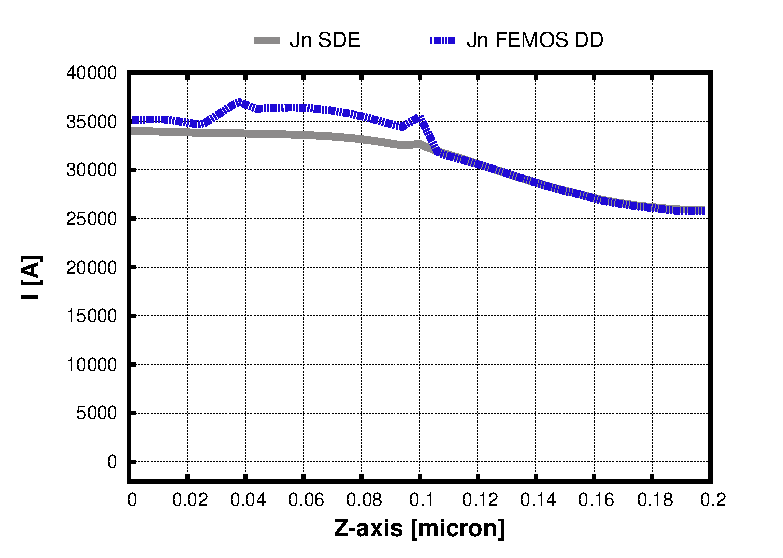
\includegraphics[width = 0.5\textwidth , height=4.5cm]{Corrente/ConfrontiCorrentiBulkJN_SDEVsDD.eps}}
\subfloat[][\emph{Standard DD - Jp}]
{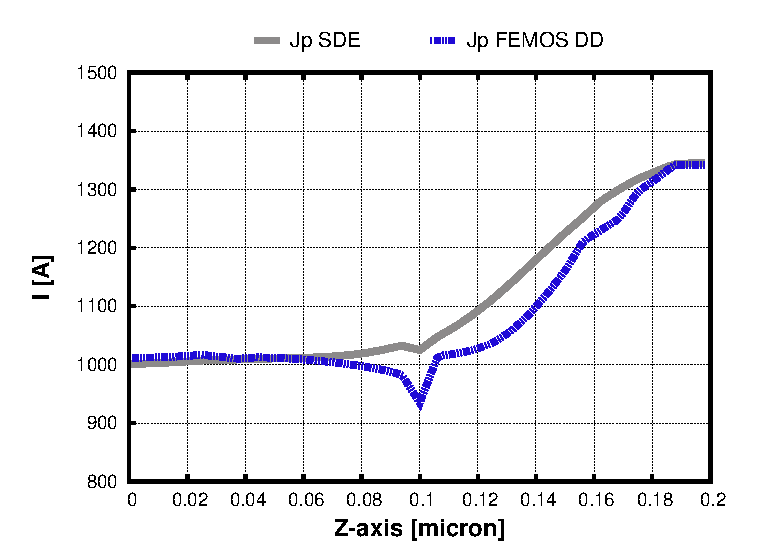
\includegraphics[width = 0.5\textwidth , height=4.5cm]{Corrente/ConfrontiCorrentiBulkJP_SDEVsDD.eps}}


\subfloat[][\emph{SG 3D - Jn}]
{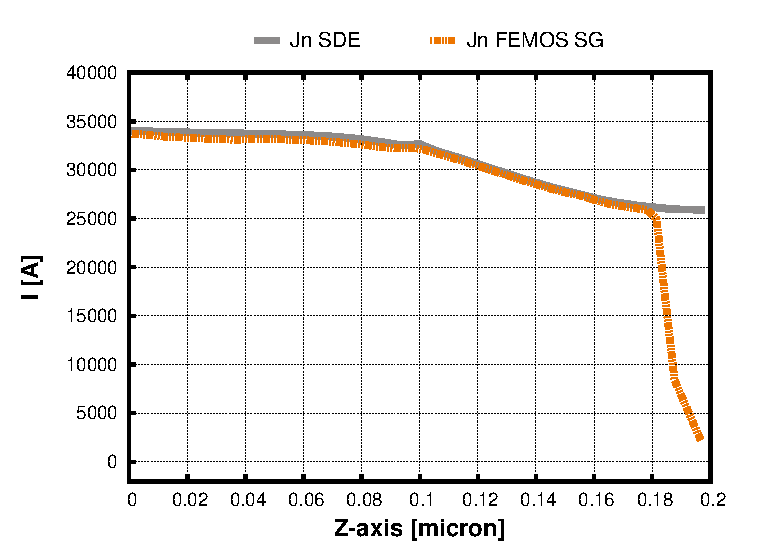
\includegraphics[width = 0.5\textwidth , height=4.5cm]{Corrente/ConfrontiCorrentiBulkJN_SDEVsSG.eps}}
\subfloat[][\emph{SG 3D - Jp}]
{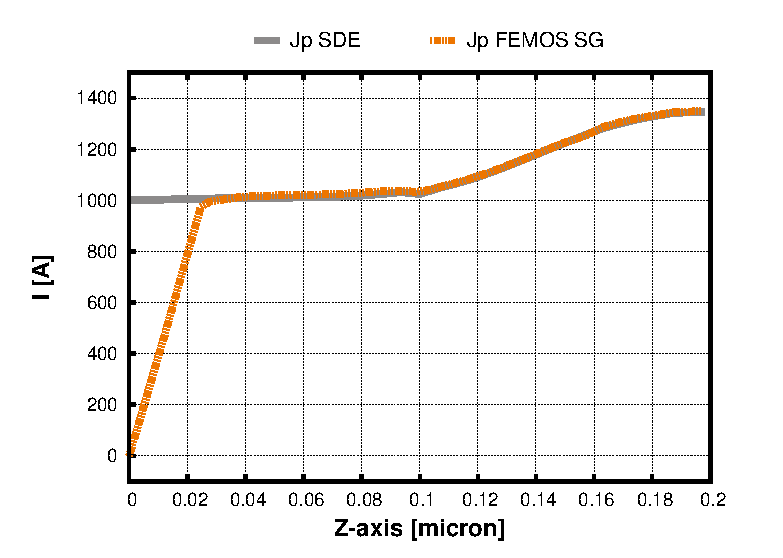
\includegraphics[width = 0.5\textwidth , height=4.5cm]{Corrente/ConfrontiCorrentiBulkJP_SDEVsSG.eps}}

\subfloat[][\emph{Modified DD - Jn}]
{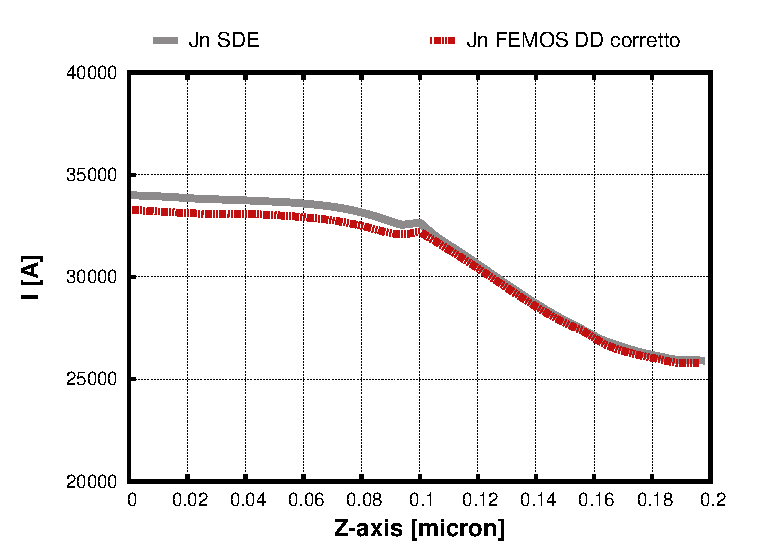
\includegraphics[width = 0.5\textwidth , height=4.5cm]{Corrente/ConfrontiCorrentiBulkJN_SDEVsDDcorretto.eps}}
\subfloat[][\emph{Modified DD - Jp}]
{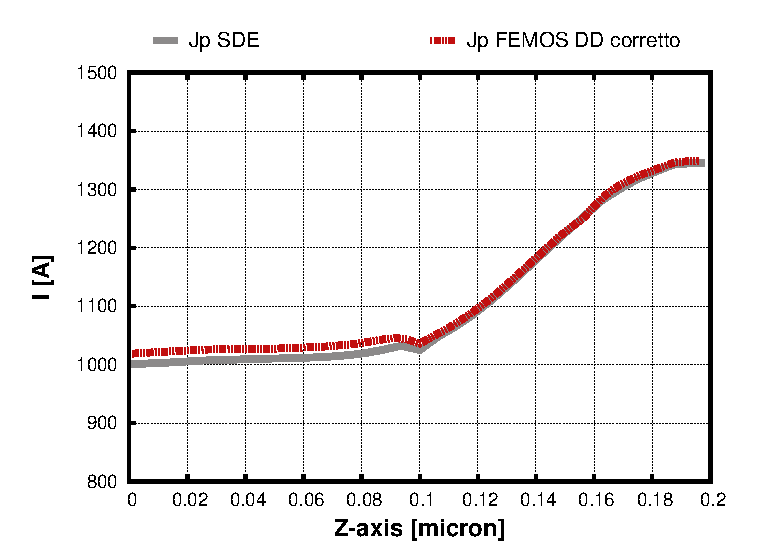
\includegraphics[width = 0.5\textwidth , height=4.5cm]{Corrente/ConfrontiCorrentiBulkJP_SDEVsDDcorretto.eps}}

\caption{1D plot p-n junction - $V_A=1.0[V]$ }
\label{fig: pn current density 1V}
\end{figure}

\textcolor{red}{Aggiungere le figure del diodo in 3D}



\begin{figure}[!h]
\centering
\subfloat[][\emph{Hole current density.}]
{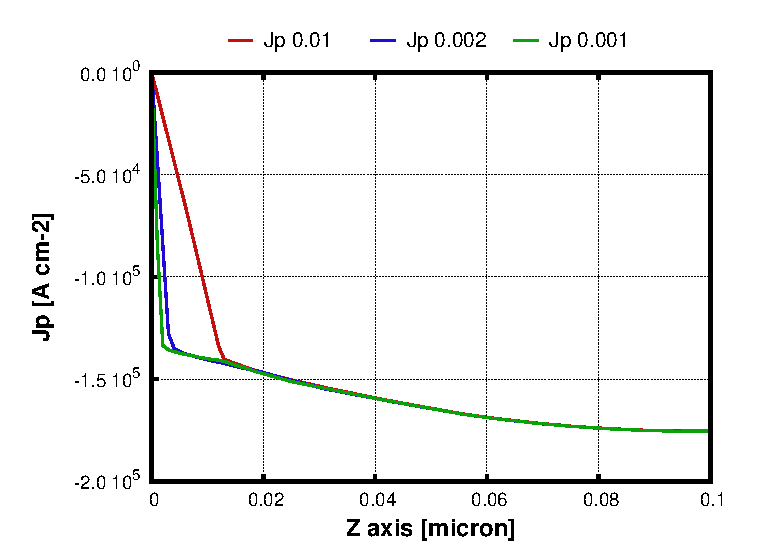
\includegraphics[width=0.5\textwidth , height=4.5cm]{DatiImmaginiTESI/Diode/ContactFiner.eps}}
\subfloat[][\emph{Hole quasi fermi potential.}]
{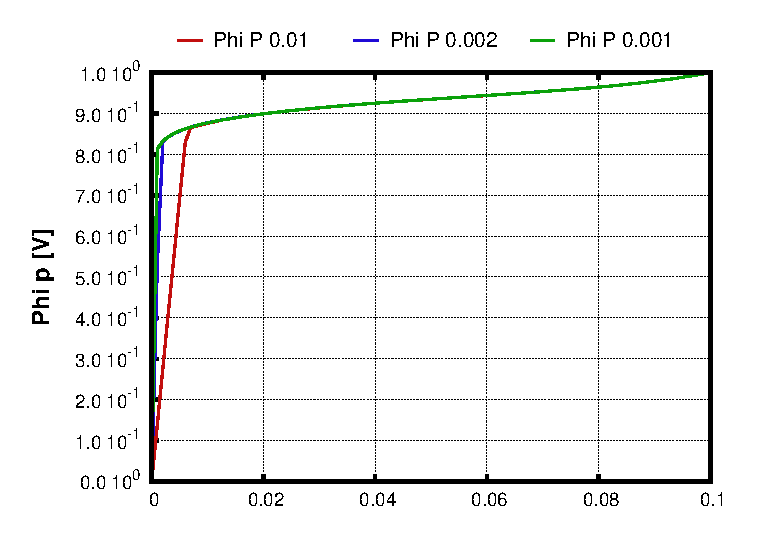
\includegraphics[width = 0.5\textwidth , height=4.5cm]{DatiImmaginiTESI/Diode/ContactFinerQFP.eps}}
\end{figure} 



%\begin{figure}[!h]
%\centering
%\subfloat[][\emph{FEMOS}]
%{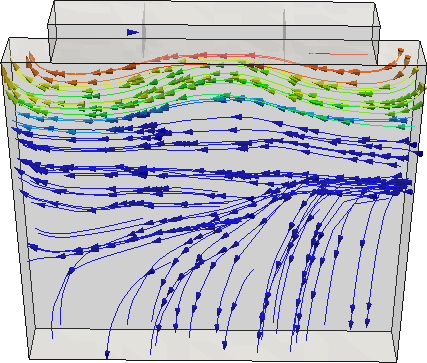
\includegraphics[scale=0.38]{Results/MOS/FEMOS181718_Jn2voltONLYDEVICE.png}}
%\hspace{0.5cm}
%\subfloat[][]
%{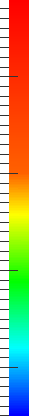
\includegraphics[scale=0.3]{Results/MOS/LegendaArcobalenoVert.png}}
%\hspace{0.5cm}
%\subfloat[][\emph{SDEVICE}]
%{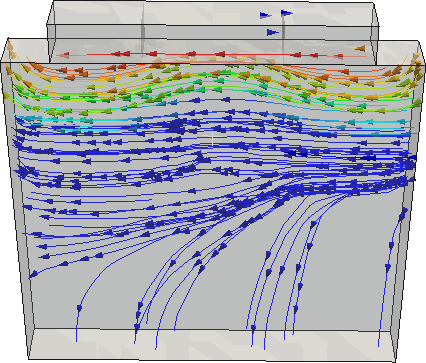
\includegraphics[scale=0.38]{Results/MOS/SDEVICE181718_Jn2voltONLYDEVICE.png}}
%\caption{Electron current density Vgate = 2.0 [V].}
%\end{figure}


When $(\varphi_{max}-\varphi_{min})$ is small or when the diode is in high direct polarization the modified technique works (\figref{fig: p-n upwinding tech}) better than the Drift-Diffusion formula (\figref{fig: p-n drift diffusion}).

\begin{figure}[!h]
\centering
\subfloat[][\emph{Jn}]
{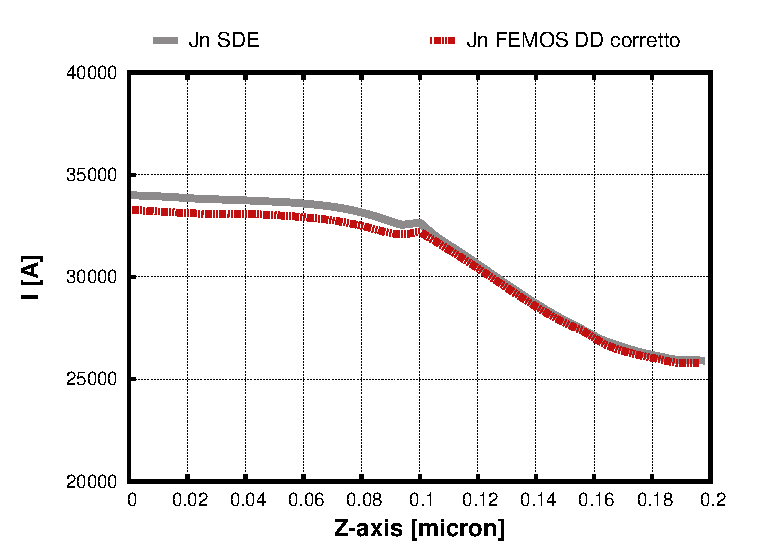
\includegraphics[width = 0.5\textwidth , height=4.5cm]{Corrente/ConfrontiCorrentiBulkJN_SDEVsDDcorretto.eps}}
\subfloat[][\emph{Jp}]
{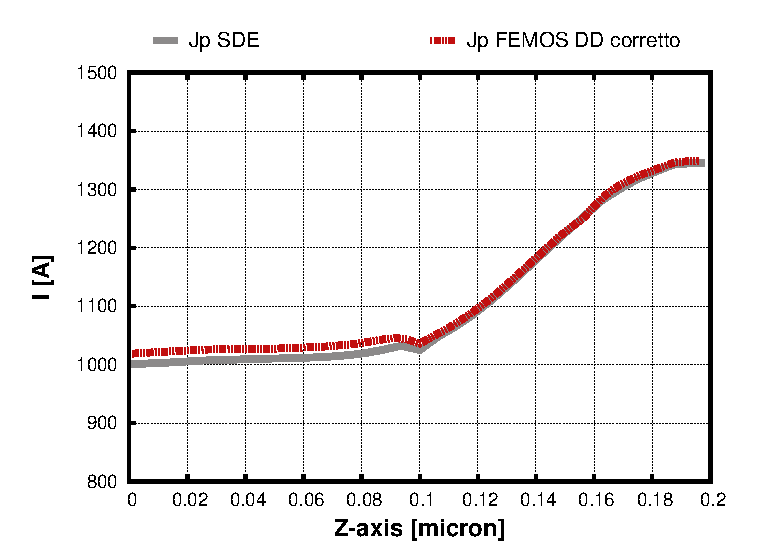
\includegraphics[width = 0.5\textwidth , height=4.5cm]{Corrente/ConfrontiCorrentiBulkJP_SDEVsDDcorretto.eps}}
\caption{1D plot p-n junction - $V_A=1.0[V]$.}
\label{fig: p-n upwinding tech}
\end{figure} 

\begin{figure}[!h]
\centering
\subfloat[][\emph{Jn}]
{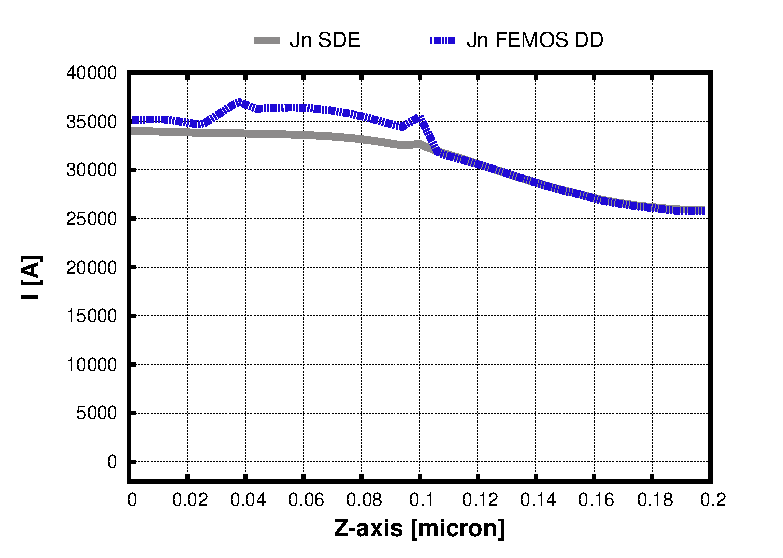
\includegraphics[width = 0.5\textwidth , height=4.5cm]{Corrente/ConfrontiCorrentiBulkJN_SDEVsDD.eps}}
\subfloat[][\emph{Jp}]
{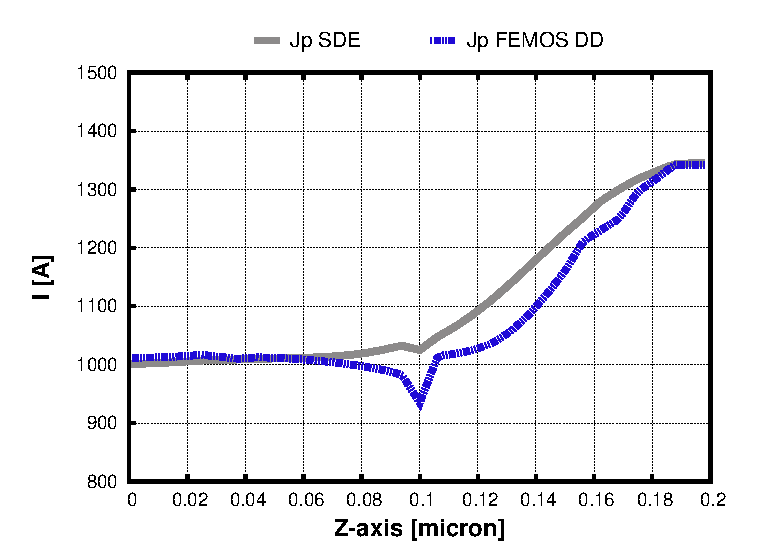
\includegraphics[width = 0.5\textwidth , height=4.5cm]{Corrente/ConfrontiCorrentiBulkJP_SDEVsDD.eps}}
\caption{1D plot p-n junction - $V_A=1.0[V]$.}
\label{fig: p-n drift diffusion}
\end{figure} 





\begin{figure}[!h]
\centering
\subfloat[][\emph{SDE}]
{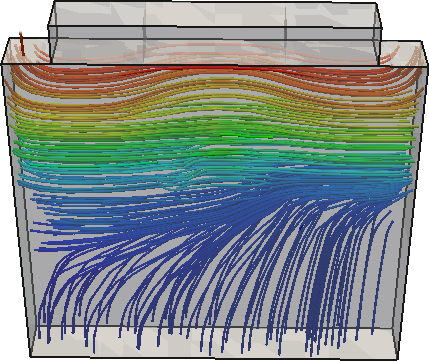
\includegraphics[width = 0.45\textwidth , height=5cm]{CapitoloCorrente/nMOS_SDE.png}}


\subfloat[][\emph{SG}]
{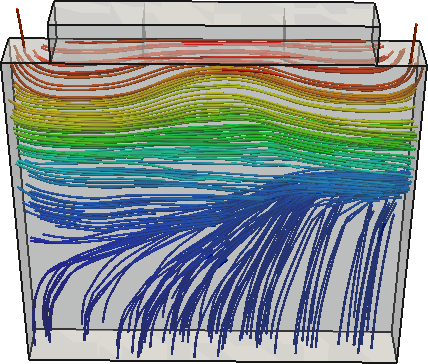
\includegraphics[width = 0.45\textwidth , height=5cm]{CapitoloCorrente/nMOS_SG_device.png}}
\hspace{0.05\textwidth}
\subfloat[][\emph{DD upwind}]
{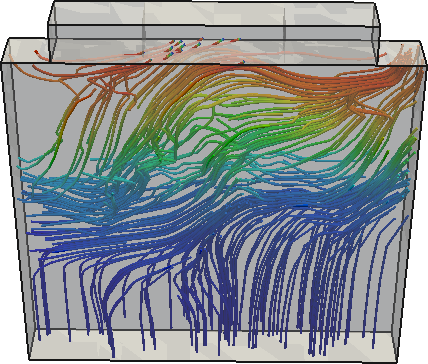
\includegraphics[width = 0.45\textwidth , height=5cm]{CapitoloCorrente/nMOS_DDcorretto.png}}

\subfloat[][\emph{DD upwind (mesh finer)}]
{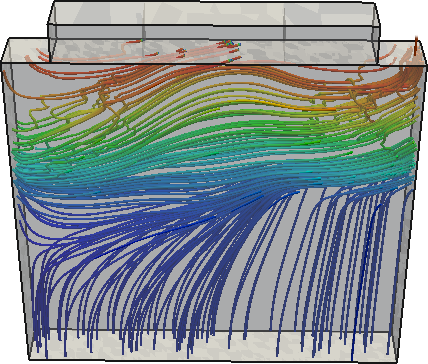
\includegraphics[width = 0.45\textwidth , height=5cm]{CapitoloCorrente/nMOS_DDcorretto35000.png}}
\hspace{0.05\textwidth}
\subfloat[][\emph{DD standard (mesh finer)}]
{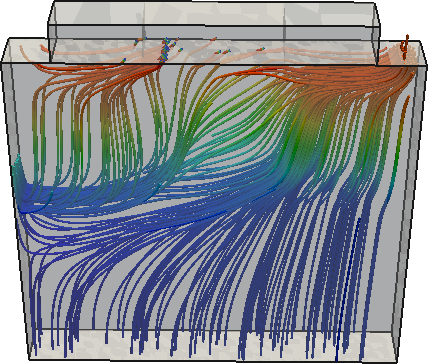
\includegraphics[width = 0.45\textwidth , height=5cm]{CapitoloCorrente/nMOS_DD35000.png}}


\caption{1D plot p-n junction - $V_A=1.0[V]$.}
\label{fig: p-n drift diffusion}
\end{figure} 